\begin{frame}
    \frametitle{Outline} 
    \tableofcontents[currentsection]
\end{frame} 

\begin{frame}
    \frametitle{Main Research Question} 

    \vspace{-0.7cm}
    \begin{center}
        \LARGE{How does VOC speciation affect\\\vspace{3mm} \ce{O3} concentrations in models?}
    \end{center}
\end{frame}

\begin{frame}
    \frametitle{Motivation}
    \begin{columns}[onlytextwidth]
        \begin{column}{0.45\textwidth}
            \begin{flushleft}
                \vspace{-1.5cm}
                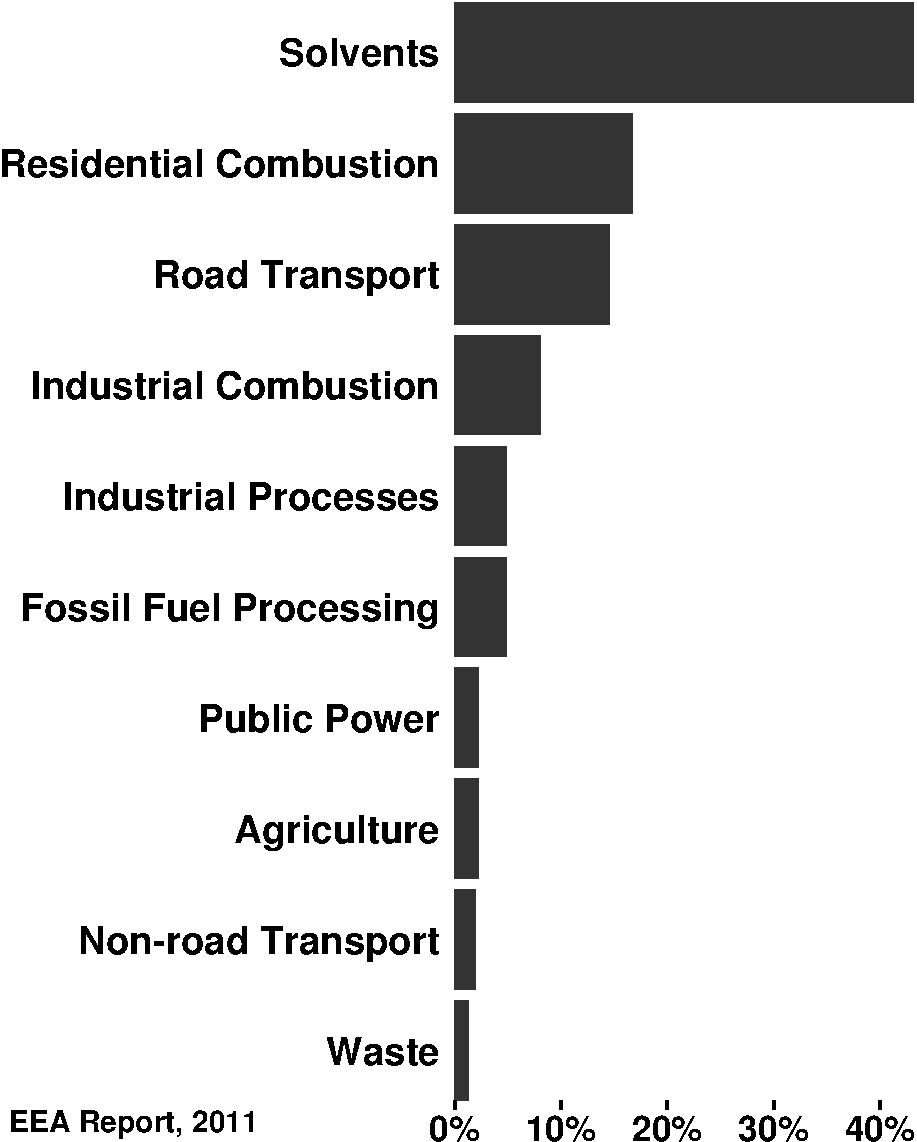
\includegraphics[width=1.10\textwidth]{../Pictures/Sector_conributions} 
            \end{flushleft}
        \end{column}%
        \begin{column}{0.45\textwidth}
            \begin{flushright}
                \vspace{-1.5cm}
                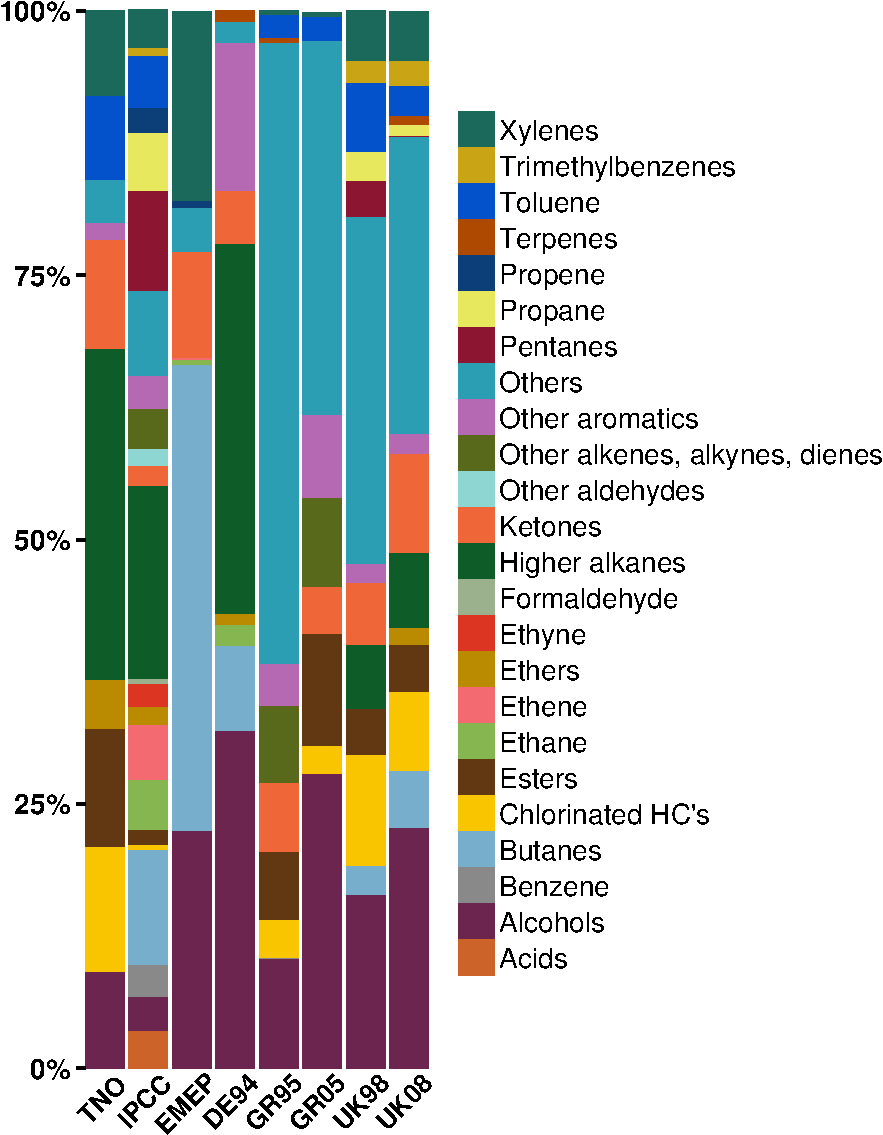
\includegraphics[width=1.10\textwidth]{../Pictures/Speciations_for_MCM} 
            \end{flushright}
        \end{column}
    \end{columns}
\end{frame}

\begin{frame}
    \frametitle{Compared Solvent Speciations}

    \vspace{-0.4cm}
    {
        \setstretch{1.15}
        \begin{table}%[!ht]
            \begin{center}
                \small\makebox[\textwidth][c]{%
                \begin{tabular}{lllP{5.2cm}}
                    \toprule
                    \textbf{Speciation} & \textbf{Reference} \\ \bottomrule
                    TNO & [Builtjes et al., TNO Report, 2002] \\ \hline
                    IPCC & [Ehhalt et al., IPCC Report, 2001] \\ \hline
                    EMEP & [Simpson et al., ACP, 2010] \\ \hline
                    DE94 & [Friedrich et. al., JAC, 2002] \\ \hline
                    GR95 & [Sidiropoulos and Tsilingiridis, FEB, 2007] \\ \hline
                    GR05 & [Sidiropoulos and Tsilingiridis, FEB, 2007] \\ \hline
                    UK98 & [Goodwin, UK NAEI report, 2000] \\ \hline
                    UK08 & [Murrells et al., UK NAEI Report, 2010] \\ \bottomrule
                \end{tabular}}
            \end{center}
        \end{table}
    }
\end{frame}

\begin{frame}
    \frametitle{Boxmodel Setup}

    \begin{itemize}
        \item MECCA boxmodel over 7 days. \vspace{5mm}
        \item Idealised urban area of 1000 km$^2$. \vspace{5mm}
        \item Total NMVOC emissions of 1000 ton/day \newline [Warnecke et al., JGR, 2007]. \vspace{5mm}
        \item NMVOC emissions constant until noon of day 1.
    \end{itemize}
\end{frame}

{
    \usebackgroundtemplate{%
        \vbox to \paperheight{\vfil\hbox to \paperwidth{\hfil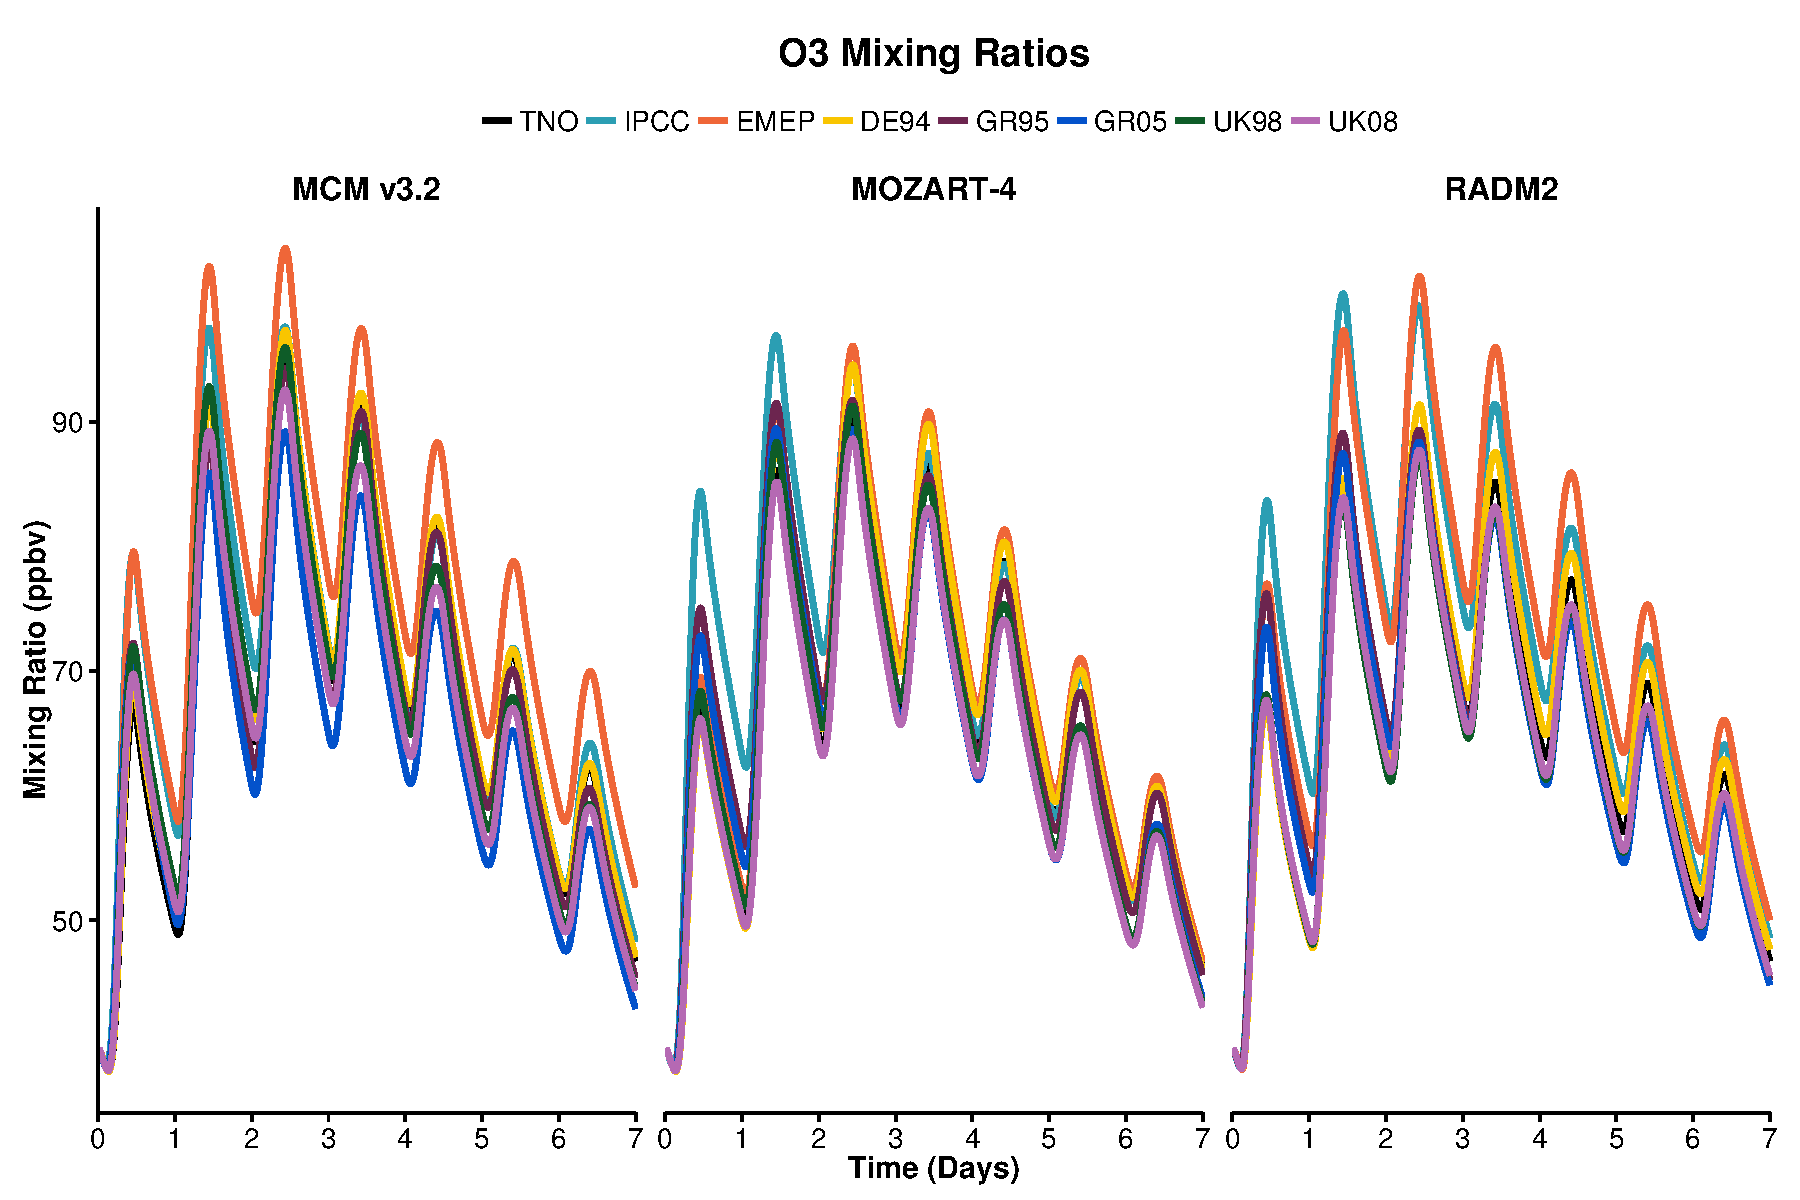
\includegraphics[height=0.90\paperheight, width = 0.98\paperwidth]{../Plotting_scripts/Solvents_Only_O3_mixing_ratios}\hfil}\vfil}
    }
    \begin{frame}[plain]
    \end{frame}
}

{
    \usebackgroundtemplate{%
        \vbox to \paperheight{\vfil\hbox to \paperwidth{\hfil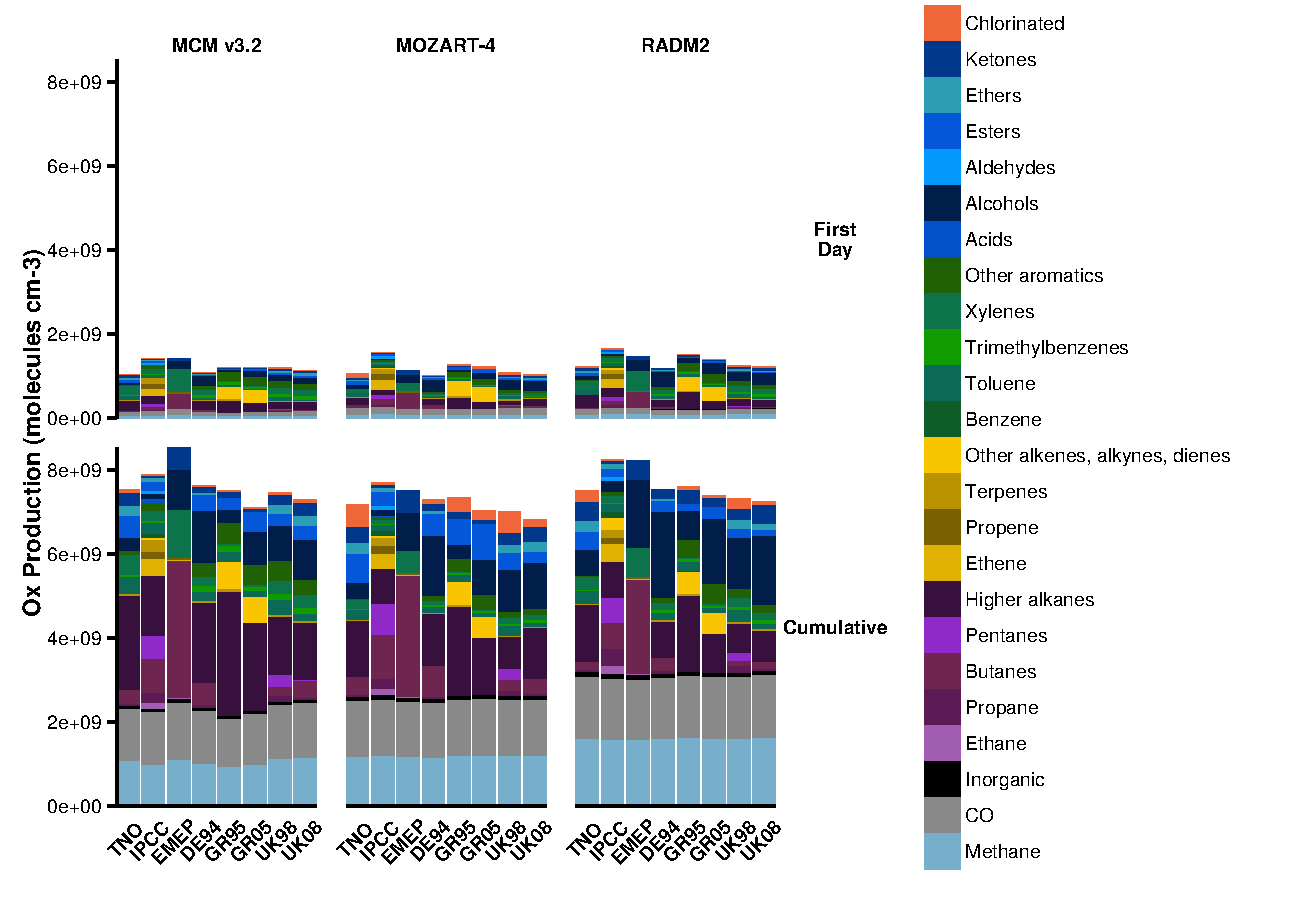
\includegraphics[height=0.98\paperheight, width = 0.98\paperwidth]{../Plotting_scripts/Absolute_Ox_budget_allocated_facet_mechanism}\hfil}\vfil}
    }
    \begin{frame}[plain]
    \end{frame}
}

{
    \usebackgroundtemplate{%
        \vbox to \paperheight{\vfil\hbox to \paperwidth{\hfil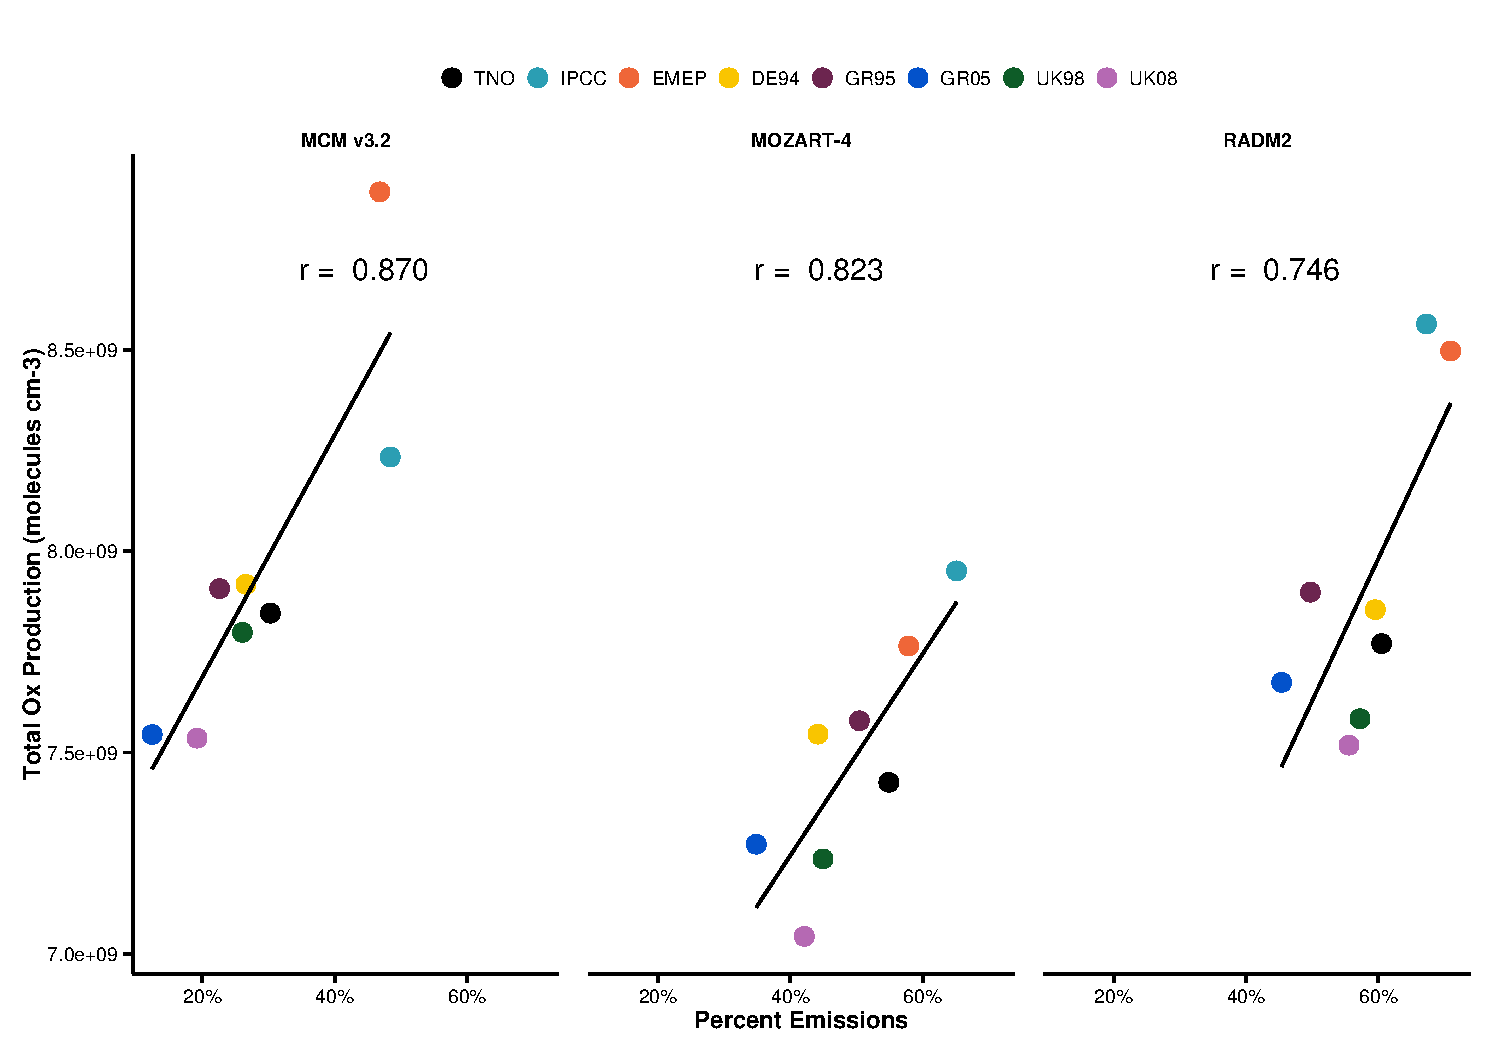
\includegraphics[height=0.98\paperheight, width = 0.98\paperwidth]{../Plotting_scripts/Ox_production_vs_type_emission_fraction_all_mechanisms}\hfil}\vfil}
    }
    \begin{frame}[plain]
    \end{frame}
}

\begin{frame}
    \frametitle{Paper Status}

    \begin{itemize}
        \item Initial draft focussing on modelling work.
        \item Erika will be first author, paper will focus on comparison of solvent sector VOC speciations performed by Erika with the modelling results supporting.
        \item Updates from Erika.
        \item Journal
        \item Deadline for submission
    \end{itemize}
\end{frame}
